\documentclass[1p]{elsarticle_modified}
%\bibliographystyle{elsarticle-num}

%\usepackage[colorlinks]{hyperref}
%\usepackage{abbrmath_seonhwa} %\Abb, \Ascr, \Acal ,\Abf, \Afrak
\usepackage{amsfonts}
\usepackage{amssymb}
\usepackage{amsmath}
\usepackage{amsthm}
\usepackage{scalefnt}
\usepackage{amsbsy}
\usepackage{kotex}
\usepackage{caption}
\usepackage{subfig}
\usepackage{color}
\usepackage{graphicx}
\usepackage{xcolor} %% white, black, red, green, blue, cyan, magenta, yellow
\usepackage{float}
\usepackage{setspace}
\usepackage{hyperref}

\usepackage{tikz}
\usetikzlibrary{arrows}

\usepackage{multirow}
\usepackage{array} % fixed length table
\usepackage{hhline}

%%%%%%%%%%%%%%%%%%%%%
\makeatletter
\renewcommand*\env@matrix[1][\arraystretch]{%
	\edef\arraystretch{#1}%
	\hskip -\arraycolsep
	\let\@ifnextchar\new@ifnextchar
	\array{*\c@MaxMatrixCols c}}
\makeatother %https://tex.stackexchange.com/questions/14071/how-can-i-increase-the-line-spacing-in-a-matrix
%%%%%%%%%%%%%%%

\usepackage[normalem]{ulem}

\newcommand{\msout}[1]{\ifmmode\text{\sout{\ensuremath{#1}}}\else\sout{#1}\fi}
%SOURCE: \msout is \stkout macro in https://tex.stackexchange.com/questions/20609/strikeout-in-math-mode

\newcommand{\cancel}[1]{
	\ifmmode
	{\color{red}\msout{#1}}
	\else
	{\color{red}\sout{#1}}
	\fi
}

\newcommand{\add}[1]{
	{\color{blue}\uwave{#1}}
}

\newcommand{\replace}[2]{
	\ifmmode
	{\color{red}\msout{#1}}{\color{blue}\uwave{#2}}
	\else
	{\color{red}\sout{#1}}{\color{blue}\uwave{#2}}
	\fi
}

\newcommand{\Sol}{\mathcal{S}} %segment
\newcommand{\D}{D} %diagram
\newcommand{\A}{\mathcal{A}} %arc


%%%%%%%%%%%%%%%%%%%%%%%%%%%%%5 test

\def\sl{\operatorname{\textup{SL}}(2,\Cbb)}
\def\psl{\operatorname{\textup{PSL}}(2,\Cbb)}
\def\quan{\mkern 1mu \triangleright \mkern 1mu}

\theoremstyle{definition}
\newtheorem{thm}{Theorem}[section]
\newtheorem{prop}[thm]{Proposition}
\newtheorem{lem}[thm]{Lemma}
\newtheorem{ques}[thm]{Question}
\newtheorem{cor}[thm]{Corollary}
\newtheorem{defn}[thm]{Definition}
\newtheorem{exam}[thm]{Example}
\newtheorem{rmk}[thm]{Remark}
\newtheorem{alg}[thm]{Algorithm}

\newcommand{\I}{\sqrt{-1}}
\begin{document}

%\begin{frontmatter}
%
%\title{Boundary parabolic representations of knots up to 8 crossings}
%
%%% Group authors per affiliation:
%\author{Yunhi Cho} 
%\address{Department of Mathematics, University of Seoul, Seoul, Korea}
%\ead{yhcho@uos.ac.kr}
%
%
%\author{Seonhwa Kim} %\fnref{s_kim}}
%\address{Center for Geometry and Physics, Institute for Basic Science, Pohang, 37673, Korea}
%\ead{ryeona17@ibs.re.kr}
%
%\author{Hyuk Kim}
%\address{Department of Mathematical Sciences, Seoul National University, Seoul 08826, Korea}
%\ead{hyukkim@snu.ac.kr}
%
%\author{Seokbeom Yoon}
%\address{Department of Mathematical Sciences, Seoul National University, Seoul, 08826,  Korea}
%\ead{sbyoon15@snu.ac.kr}
%
%\begin{abstract}
%We find all boundary parabolic representation of knots up to 8 crossings.
%
%\end{abstract}
%\begin{keyword}
%    \MSC[2010] 57M25 
%\end{keyword}
%
%\end{frontmatter}

%\linenumbers
%\tableofcontents
%
\newcommand\colored[1]{\textcolor{white}{\rule[-0.35ex]{0.8em}{1.4ex}}\kern-0.8em\color{red} #1}%
%\newcommand\colored[1]{\textcolor{white}{ #1}\kern-2.17ex	\textcolor{white}{ #1}\kern-1.81ex	\textcolor{white}{ #1}\kern-2.15ex\color{red}#1	}

{\Large $\underline{11n_{33}~(K11n_{33})}$}

\setlength{\tabcolsep}{10pt}
\renewcommand{\arraystretch}{1.6}
\vspace{1cm}\begin{tabular}{m{100pt}>{\centering\arraybackslash}m{274pt}}
\multirow{5}{120pt}{
	\centering
	\includegraphics[width=112pt]{../../../GIT/diagram.site/Diagrams/png/649_11n_33.png}\\
\ \ \ A knot diagram\footnotemark}&
\allowdisplaybreaks
\textbf{Linearized knot diagam} \\
\cline{2-2}
 &
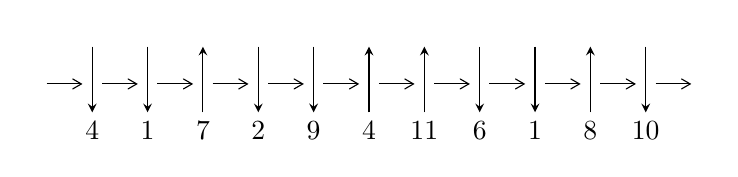
\begin{tikzpicture}[x=20pt, y=17pt]
	% nodes
	\node (C0) at (0, 0) {};
	\node (C1) at (1, 0) {};
	\node (C1U) at (1, +1) {};
	\node (C1D) at (1, -1) {4};

	\node (C2) at (2, 0) {};
	\node (C2U) at (2, +1) {};
	\node (C2D) at (2, -1) {1};

	\node (C3) at (3, 0) {};
	\node (C3U) at (3, +1) {};
	\node (C3D) at (3, -1) {7};

	\node (C4) at (4, 0) {};
	\node (C4U) at (4, +1) {};
	\node (C4D) at (4, -1) {2};

	\node (C5) at (5, 0) {};
	\node (C5U) at (5, +1) {};
	\node (C5D) at (5, -1) {9};

	\node (C6) at (6, 0) {};
	\node (C6U) at (6, +1) {};
	\node (C6D) at (6, -1) {4};

	\node (C7) at (7, 0) {};
	\node (C7U) at (7, +1) {};
	\node (C7D) at (7, -1) {11};

	\node (C8) at (8, 0) {};
	\node (C8U) at (8, +1) {};
	\node (C8D) at (8, -1) {6};

	\node (C9) at (9, 0) {};
	\node (C9U) at (9, +1) {};
	\node (C9D) at (9, -1) {1};

	\node (C10) at (10, 0) {};
	\node (C10U) at (10, +1) {};
	\node (C10D) at (10, -1) {8};

	\node (C11) at (11, 0) {};
	\node (C11U) at (11, +1) {};
	\node (C11D) at (11, -1) {10};
	\node (C12) at (12, 0) {};

	% arrows
	\draw[->,>={angle 60}]
	(C0) edge (C1) (C1) edge (C2) (C2) edge (C3) (C3) edge (C4) (C4) edge (C5) (C5) edge (C6) (C6) edge (C7) (C7) edge (C8) (C8) edge (C9) (C9) edge (C10) (C10) edge (C11) (C11) edge (C12) ;	\draw[->,>=stealth]
	(C1U) edge (C1D) (C2U) edge (C2D) (C3D) edge (C3U) (C4U) edge (C4D) (C5U) edge (C5D) (C6D) edge (C6U) (C7D) edge (C7U) (C8U) edge (C8D) (C9U) edge (C9D) (C10D) edge (C10U) (C11U) edge (C11D) ;
	\end{tikzpicture} \\
\hhline{~~} \\& 
\textbf{Solving Sequence} \\ \cline{2-2} 
 &
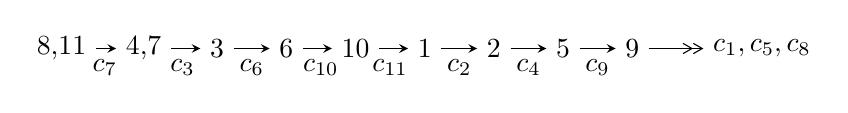
\begin{tikzpicture}[x=25pt, y=7pt]
	% node
	\node (A0) at (-1/8, 0) {8,11};
	\node (A1) at (17/16, 0) {4,7};
	\node (A2) at (17/8, 0) {3};
	\node (A3) at (25/8, 0) {6};
	\node (A4) at (33/8, 0) {10};
	\node (A5) at (41/8, 0) {1};
	\node (A6) at (49/8, 0) {2};
	\node (A7) at (57/8, 0) {5};
	\node (A8) at (65/8, 0) {9};
	\node (C1) at (1/2, -1) {$c_{7}$};
	\node (C2) at (13/8, -1) {$c_{3}$};
	\node (C3) at (21/8, -1) {$c_{6}$};
	\node (C4) at (29/8, -1) {$c_{10}$};
	\node (C5) at (37/8, -1) {$c_{11}$};
	\node (C6) at (45/8, -1) {$c_{2}$};
	\node (C7) at (53/8, -1) {$c_{4}$};
	\node (C8) at (61/8, -1) {$c_{9}$};
	\node (A9) at (10, 0) {$c_{1},c_{5},c_{8}$};

	% edge
	\draw[->,>=stealth]	
	(A0) edge (A1) (A1) edge (A2) (A2) edge (A3) (A3) edge (A4) (A4) edge (A5) (A5) edge (A6) (A6) edge (A7) (A7) edge (A8) ;
	\draw[->>,>={angle 60}]	
	(A8) edge (A9);
\end{tikzpicture} \\ 

\end{tabular} \\

\footnotetext{
The image of knot diagram is generated by the software ``\textbf{Draw programme}" developed by Andrew Bartholomew(\url{http://www.layer8.co.uk/maths/draw/index.htm\#Running-draw}), where we modified some parts for our purpose(\url{https://github.com/CATsTAILs/LinksPainter}).
}\phantom \\ \newline 
\centering \textbf{Ideals for irreducible components\footnotemark of $X_{\text{par}}$} 
 
\begin{align*}
I^u_{1}&=\langle 
-37402427 u^{28}+81134437 u^{27}+\cdots+95729774 b+19128061,\\
\phantom{I^u_{1}}&\phantom{= \langle  }18654994 u^{28}-22307356 u^{27}+\cdots+47864887 a+114512378,\;u^{29}-2 u^{28}+\cdots+3 u-1\rangle \\
I^u_{2}&=\langle 
- u^2+b+u-1,\;- u^3+2 u^2+a-2 u,\;u^4- u^3+u^2+1\rangle \\
\\
\end{align*}
\raggedright * 2 irreducible components of $\dim_{\mathbb{C}}=0$, with total 33 representations.\\
\footnotetext{All coefficients of polynomials are rational numbers. But the coefficients are sometimes approximated in decimal forms when there is not enough margin.}
\newpage
\renewcommand{\arraystretch}{1}
\centering \section*{I. $I^u_{1}= \langle -3.74\times10^{7} u^{28}+8.11\times10^{7} u^{27}+\cdots+9.57\times10^{7} b+1.91\times10^{7},\;1.87\times10^{7} u^{28}-2.23\times10^{7} u^{27}+\cdots+4.79\times10^{7} a+1.15\times10^{8},\;u^{29}-2 u^{28}+\cdots+3 u-1 \rangle$}
\flushleft \textbf{(i) Arc colorings}\\
\begin{tabular}{m{7pt} m{180pt} m{7pt} m{180pt} }
\flushright $a_{8}=$&$\begin{pmatrix}1\\0\end{pmatrix}$ \\
\flushright $a_{11}=$&$\begin{pmatrix}0\\u\end{pmatrix}$ \\
\flushright $a_{4}=$&$\begin{pmatrix}-0.389743 u^{28}+0.466048 u^{27}+\cdots-0.0720082 u-2.39241\\0.390708 u^{28}-0.847536 u^{27}+\cdots+1.96725 u-0.199813\end{pmatrix}$ \\
\flushright $a_{7}=$&$\begin{pmatrix}1\\u^2\end{pmatrix}$ \\
\flushright $a_{3}=$&$\begin{pmatrix}-0.301913 u^{28}+0.291851 u^{27}+\cdots-1.48869 u-2.50603\\0.301774 u^{28}-0.697679 u^{27}+\cdots+2.05069 u-0.198352\end{pmatrix}$ \\
\flushright $a_{6}=$&$\begin{pmatrix}-0.387941 u^{28}+0.329624 u^{27}+\cdots-1.28229 u-0.468247\\-0.00769895 u^{28}+0.202551 u^{27}+\cdots-0.868360 u+0.400024\end{pmatrix}$ \\
\flushright $a_{10}=$&$\begin{pmatrix}- u\\u\end{pmatrix}$ \\
\flushright $a_{1}=$&$\begin{pmatrix}- u^3\\u^3+u\end{pmatrix}$ \\
\flushright $a_{2}=$&$\begin{pmatrix}-0.613206 u^{28}+0.567015 u^{27}+\cdots-1.46731 u-2.44550\\0.410088 u^{28}-0.627420 u^{27}+\cdots+2.11495 u-0.000268506\end{pmatrix}$ \\
\flushright $a_{5}=$&$\begin{pmatrix}0.380897 u^{28}+0.633142 u^{27}+\cdots+3.45405 u-0.121313\\0.0116806 u^{28}-0.577333 u^{27}+\cdots+0.279345 u-0.400432\end{pmatrix}$ \\
\flushright $a_{9}=$&$\begin{pmatrix}- u^5- u\\u^5+u^3+u\end{pmatrix}$\\ \flushright $a_{9}=$&$\begin{pmatrix}- u^5- u\\u^5+u^3+u\end{pmatrix}$\\&\end{tabular}
\flushleft \textbf{(ii) Obstruction class $= -1$}\\~\\
\flushleft \textbf{(iii) Cusp Shapes $= \frac{65937967}{47864887} u^{28}-\frac{91712198}{47864887} u^{27}+\cdots+\frac{129153968}{47864887} u-\frac{217380957}{47864887}$}\\~\\
\newpage\renewcommand{\arraystretch}{1}
\flushleft \textbf{(iv) u-Polynomials at the component}\newline \\
\begin{tabular}{m{50pt}|m{274pt}}
Crossings & \hspace{64pt}u-Polynomials at each crossing \\
\hline $$\begin{aligned}c_{1},c_{4}\end{aligned}$$&$\begin{aligned}
&u^{29}-5 u^{28}+\cdots+11 u+1
\end{aligned}$\\
\hline $$\begin{aligned}c_{2}\end{aligned}$$&$\begin{aligned}
&u^{29}+33 u^{28}+\cdots+5 u+1
\end{aligned}$\\
\hline $$\begin{aligned}c_{3},c_{6}\end{aligned}$$&$\begin{aligned}
&u^{29}+5 u^{28}+\cdots-72 u+16
\end{aligned}$\\
\hline $$\begin{aligned}c_{5},c_{8}\end{aligned}$$&$\begin{aligned}
&u^{29}-2 u^{28}+\cdots+u-1
\end{aligned}$\\
\hline $$\begin{aligned}c_{7},c_{10}\end{aligned}$$&$\begin{aligned}
&u^{29}+2 u^{28}+\cdots+3 u+1
\end{aligned}$\\
\hline $$\begin{aligned}c_{9},c_{11}\end{aligned}$$&$\begin{aligned}
&u^{29}+12 u^{28}+\cdots- u-1
\end{aligned}$\\
\hline
\end{tabular}\\~\\
\newpage\renewcommand{\arraystretch}{1}
\flushleft \textbf{(v) Riley Polynomials at the component}\newline \\
\begin{tabular}{m{50pt}|m{274pt}}
Crossings & \hspace{64pt}Riley Polynomials at each crossing \\
\hline $$\begin{aligned}c_{1},c_{4}\end{aligned}$$&$\begin{aligned}
&y^{29}-33 y^{28}+\cdots+5 y-1
\end{aligned}$\\
\hline $$\begin{aligned}c_{2}\end{aligned}$$&$\begin{aligned}
&y^{29}-69 y^{28}+\cdots-1359 y-1
\end{aligned}$\\
\hline $$\begin{aligned}c_{3},c_{6}\end{aligned}$$&$\begin{aligned}
&y^{29}+27 y^{28}+\cdots-2240 y-256
\end{aligned}$\\
\hline $$\begin{aligned}c_{5},c_{8}\end{aligned}$$&$\begin{aligned}
&y^{29}+30 y^{27}+\cdots- y-1
\end{aligned}$\\
\hline $$\begin{aligned}c_{7},c_{10}\end{aligned}$$&$\begin{aligned}
&y^{29}+12 y^{28}+\cdots- y-1
\end{aligned}$\\
\hline $$\begin{aligned}c_{9},c_{11}\end{aligned}$$&$\begin{aligned}
&y^{29}+12 y^{28}+\cdots+35 y-1
\end{aligned}$\\
\hline
\end{tabular}\\~\\
\newpage\flushleft \textbf{(vi) Complex Volumes and Cusp Shapes}
$$\begin{array}{c|c|c}  
\text{Solutions to }I^u_{1}& \I (\text{vol} + \sqrt{-1}CS) & \text{Cusp shape}\\
 \hline 
\begin{aligned}
u &= -0.430937 + 0.875588 I \\
a &= \phantom{-}2.46856 + 2.58292 I \\
b &= \phantom{-}0.13985 - 3.12093 I\end{aligned}
 & -1.94857 - 1.79081 I & \phantom{-}9.7159 + 22.2862 I \\ \hline\begin{aligned}
u &= -0.430937 - 0.875588 I \\
a &= \phantom{-}2.46856 - 2.58292 I \\
b &= \phantom{-}0.13985 + 3.12093 I\end{aligned}
 & -1.94857 + 1.79081 I & \phantom{-}9.7159 - 22.2862 I \\ \hline\begin{aligned}
u &= \phantom{-}0.251301 + 0.941534 I \\
a &= -1.04299 + 2.34476 I \\
b &= \phantom{-}0.283465 - 0.998451 I\end{aligned}
 & -3.57724 - 0.66247 I & -10.09352 + 1.94504 I \\ \hline\begin{aligned}
u &= \phantom{-}0.251301 - 0.941534 I \\
a &= -1.04299 - 2.34476 I \\
b &= \phantom{-}0.283465 + 0.998451 I\end{aligned}
 & -3.57724 + 0.66247 I & -10.09352 - 1.94504 I \\ \hline\begin{aligned}
u &= \phantom{-}0.932586 + 0.472277 I \\
a &= -0.0835356 + 0.0913296 I \\
b &= \phantom{-}0.58205 - 1.50292 I\end{aligned}
 & -6.37168 - 6.75282 I & -3.69355 + 3.15214 I \\ \hline\begin{aligned}
u &= \phantom{-}0.932586 - 0.472277 I \\
a &= -0.0835356 - 0.0913296 I \\
b &= \phantom{-}0.58205 + 1.50292 I\end{aligned}
 & -6.37168 + 6.75282 I & -3.69355 - 3.15214 I \\ \hline\begin{aligned}
u &= -0.953647 + 0.505885 I \\
a &= -0.0879207 + 0.0911589 I \\
b &= \phantom{-}0.085199 - 1.281550 I\end{aligned}
 & -6.12495 - 1.71894 I & -4.74605 + 1.89417 I \\ \hline\begin{aligned}
u &= -0.953647 - 0.505885 I \\
a &= -0.0879207 - 0.0911589 I \\
b &= \phantom{-}0.085199 + 1.281550 I\end{aligned}
 & -6.12495 + 1.71894 I & -4.74605 - 1.89417 I \\ \hline\begin{aligned}
u &= -0.547094 + 0.958808 I \\
a &= -1.29758 - 1.42753 I \\
b &= -0.64604 + 1.52374 I\end{aligned}
 & -0.84435 - 2.90824 I & -4.00553 + 0.79959 I \\ \hline\begin{aligned}
u &= -0.547094 - 0.958808 I \\
a &= -1.29758 + 1.42753 I \\
b &= -0.64604 - 1.52374 I\end{aligned}
 & -0.84435 + 2.90824 I & -4.00553 - 0.79959 I\\
 \hline 
 \end{array}$$\newpage$$\begin{array}{c|c|c}  
\text{Solutions to }I^u_{1}& \I (\text{vol} + \sqrt{-1}CS) & \text{Cusp shape}\\
 \hline 
\begin{aligned}
u &= \phantom{-}0.429919 + 1.019430 I \\
a &= \phantom{-}1.079660 + 0.824021 I \\
b &= \phantom{-}0.147997 - 0.384192 I\end{aligned}
 & -4.75773 + 3.16768 I & -10.84320 - 4.60951 I \\ \hline\begin{aligned}
u &= \phantom{-}0.429919 - 1.019430 I \\
a &= \phantom{-}1.079660 - 0.824021 I \\
b &= \phantom{-}0.147997 + 0.384192 I\end{aligned}
 & -4.75773 - 3.16768 I & -10.84320 + 4.60951 I \\ \hline\begin{aligned}
u &= -0.493784 + 0.719618 I \\
a &= -0.524927 + 0.358431 I \\
b &= \phantom{-}0.543180 + 0.690761 I\end{aligned}
 & \phantom{-}0.00011 - 1.41557 I & -1.83013 + 4.50450 I \\ \hline\begin{aligned}
u &= -0.493784 - 0.719618 I \\
a &= -0.524927 - 0.358431 I \\
b &= \phantom{-}0.543180 - 0.690761 I\end{aligned}
 & \phantom{-}0.00011 + 1.41557 I & -1.83013 - 4.50450 I \\ \hline\begin{aligned}
u &= \phantom{-}0.559884 + 1.035720 I \\
a &= \phantom{-}1.24254 - 1.84489 I \\
b &= \phantom{-}0.620348 + 1.095660 I\end{aligned}
 & -1.53843 + 6.72020 I & -5.08320 - 8.59362 I \\ \hline\begin{aligned}
u &= \phantom{-}0.559884 - 1.035720 I \\
a &= \phantom{-}1.24254 + 1.84489 I \\
b &= \phantom{-}0.620348 - 1.095660 I\end{aligned}
 & -1.53843 - 6.72020 I & -5.08320 + 8.59362 I \\ \hline\begin{aligned}
u &= \phantom{-}0.819034 + 0.903920 I \\
a &= \phantom{-}0.003538 - 0.368412 I \\
b &= -0.0535027 + 0.0855444 I\end{aligned}
 & \phantom{-}5.64977 + 3.06577 I & \phantom{-}7.92754 - 1.40495 I \\ \hline\begin{aligned}
u &= \phantom{-}0.819034 - 0.903920 I \\
a &= \phantom{-}0.003538 + 0.368412 I \\
b &= -0.0535027 - 0.0855444 I\end{aligned}
 & \phantom{-}5.64977 - 3.06577 I & \phantom{-}7.92754 + 1.40495 I \\ \hline\begin{aligned}
u &= \phantom{-}0.591123 + 0.479483 I \\
a &= -0.544559 - 0.113805 I \\
b &= -0.539946 + 0.901812 I\end{aligned}
 & \phantom{-}0.05591 - 2.10154 I & -1.15823 + 3.97516 I \\ \hline\begin{aligned}
u &= \phantom{-}0.591123 - 0.479483 I \\
a &= -0.544559 + 0.113805 I \\
b &= -0.539946 - 0.901812 I\end{aligned}
 & \phantom{-}0.05591 + 2.10154 I & -1.15823 - 3.97516 I\\
 \hline 
 \end{array}$$\newpage$$\begin{array}{c|c|c}  
\text{Solutions to }I^u_{1}& \I (\text{vol} + \sqrt{-1}CS) & \text{Cusp shape}\\
 \hline 
\begin{aligned}
u &= \phantom{-}0.011422 + 1.270990 I \\
a &= \phantom{-}0.43345 - 2.08872 I \\
b &= -0.25247 + 1.62101 I\end{aligned}
 & -12.90150 - 4.17591 I & -8.75836 + 2.29339 I \\ \hline\begin{aligned}
u &= \phantom{-}0.011422 - 1.270990 I \\
a &= \phantom{-}0.43345 + 2.08872 I \\
b &= -0.25247 - 1.62101 I\end{aligned}
 & -12.90150 + 4.17591 I & -8.75836 - 2.29339 I \\ \hline\begin{aligned}
u &= \phantom{-}0.672968 + 1.141060 I \\
a &= -1.17654 + 1.68782 I \\
b &= -0.69150 - 1.64363 I\end{aligned}
 & -8.4308 + 12.6362 I & -5.52931 - 7.07301 I \\ \hline\begin{aligned}
u &= \phantom{-}0.672968 - 1.141060 I \\
a &= -1.17654 - 1.68782 I \\
b &= -0.69150 + 1.64363 I\end{aligned}
 & -8.4308 - 12.6362 I & -5.52931 + 7.07301 I \\ \hline\begin{aligned}
u &= -0.692012 + 1.147210 I \\
a &= \phantom{-}1.31632 + 0.88452 I \\
b &= \phantom{-}0.117471 - 1.304600 I\end{aligned}
 & -8.11998 - 4.31757 I & -6.45074 + 2.65761 I \\ \hline\begin{aligned}
u &= -0.692012 - 1.147210 I \\
a &= \phantom{-}1.31632 - 0.88452 I \\
b &= \phantom{-}0.117471 + 1.304600 I\end{aligned}
 & -8.11998 + 4.31757 I & -6.45074 - 2.65761 I \\ \hline\begin{aligned}
u &= -0.332179 + 0.485836 I \\
a &= -0.663603 + 0.306233 I \\
b &= -0.103350 + 0.657057 I\end{aligned}
 & \phantom{-}0.002667 - 1.254980 I & -0.07638 + 5.17093 I \\ \hline\begin{aligned}
u &= -0.332179 - 0.485836 I \\
a &= -0.663603 - 0.306233 I \\
b &= -0.103350 - 0.657057 I\end{aligned}
 & \phantom{-}0.002667 + 1.254980 I & -0.07638 - 5.17093 I \\ \hline\begin{aligned}
u &= \phantom{-}0.362835\phantom{ +0.000000I} \\
a &= -3.24481\phantom{ +0.000000I} \\
b &= \phantom{-}0.534503\phantom{ +0.000000I}\end{aligned}
 & -2.52742\phantom{ +0.000000I} & -3.75050\phantom{ +0.000000I}\\
 \hline 
 \end{array}$$\newpage\newpage\renewcommand{\arraystretch}{1}
\centering \section*{II. $I^u_{2}= \langle - u^2+b+u-1,\;- u^3+2 u^2+a-2 u,\;u^4- u^3+u^2+1 \rangle$}
\flushleft \textbf{(i) Arc colorings}\\
\begin{tabular}{m{7pt} m{180pt} m{7pt} m{180pt} }
\flushright $a_{8}=$&$\begin{pmatrix}1\\0\end{pmatrix}$ \\
\flushright $a_{11}=$&$\begin{pmatrix}0\\u\end{pmatrix}$ \\
\flushright $a_{4}=$&$\begin{pmatrix}u^3-2 u^2+2 u\\u^2- u+1\end{pmatrix}$ \\
\flushright $a_{7}=$&$\begin{pmatrix}1\\u^2\end{pmatrix}$ \\
\flushright $a_{3}=$&$\begin{pmatrix}u^3-2 u^2+2 u\\u^2- u+1\end{pmatrix}$ \\
\flushright $a_{6}=$&$\begin{pmatrix}1\\u^2\end{pmatrix}$ \\
\flushright $a_{10}=$&$\begin{pmatrix}- u\\u\end{pmatrix}$ \\
\flushright $a_{1}=$&$\begin{pmatrix}- u^3\\u^3+u\end{pmatrix}$ \\
\flushright $a_{2}=$&$\begin{pmatrix}-2 u^2+2 u\\u^3+u^2+1\end{pmatrix}$ \\
\flushright $a_{5}=$&$\begin{pmatrix}u^3\\- u^3- u\end{pmatrix}$ \\
\flushright $a_{9}=$&$\begin{pmatrix}u^2+1\\u^3- u^2-1\end{pmatrix}$\\ \flushright $a_{9}=$&$\begin{pmatrix}u^2+1\\u^3- u^2-1\end{pmatrix}$\\&\end{tabular}
\flushleft \textbf{(ii) Obstruction class $= 1$}\\~\\
\flushleft \textbf{(iii) Cusp Shapes $= 3 u^3-5 u^2-4$}\\~\\
\newpage\renewcommand{\arraystretch}{1}
\flushleft \textbf{(iv) u-Polynomials at the component}\newline \\
\begin{tabular}{m{50pt}|m{274pt}}
Crossings & \hspace{64pt}u-Polynomials at each crossing \\
\hline $$\begin{aligned}c_{1}\end{aligned}$$&$\begin{aligned}
&(u-1)^4
\end{aligned}$\\
\hline $$\begin{aligned}c_{2},c_{4}\end{aligned}$$&$\begin{aligned}
&(u+1)^4
\end{aligned}$\\
\hline $$\begin{aligned}c_{3},c_{6}\end{aligned}$$&$\begin{aligned}
&u^4
\end{aligned}$\\
\hline $$\begin{aligned}c_{5},c_{9}\end{aligned}$$&$\begin{aligned}
&u^4- u^3+3 u^2-2 u+1
\end{aligned}$\\
\hline $$\begin{aligned}c_{7}\end{aligned}$$&$\begin{aligned}
&u^4- u^3+u^2+1
\end{aligned}$\\
\hline $$\begin{aligned}c_{8},c_{11}\end{aligned}$$&$\begin{aligned}
&u^4+u^3+3 u^2+2 u+1
\end{aligned}$\\
\hline $$\begin{aligned}c_{10}\end{aligned}$$&$\begin{aligned}
&u^4+u^3+u^2+1
\end{aligned}$\\
\hline
\end{tabular}\\~\\
\newpage\renewcommand{\arraystretch}{1}
\flushleft \textbf{(v) Riley Polynomials at the component}\newline \\
\begin{tabular}{m{50pt}|m{274pt}}
Crossings & \hspace{64pt}Riley Polynomials at each crossing \\
\hline $$\begin{aligned}c_{1},c_{2},c_{4}\end{aligned}$$&$\begin{aligned}
&(y-1)^4
\end{aligned}$\\
\hline $$\begin{aligned}c_{3},c_{6}\end{aligned}$$&$\begin{aligned}
&y^4
\end{aligned}$\\
\hline $$\begin{aligned}c_{5},c_{8},c_{9}\\c_{11}\end{aligned}$$&$\begin{aligned}
&y^4+5 y^3+7 y^2+2 y+1
\end{aligned}$\\
\hline $$\begin{aligned}c_{7},c_{10}\end{aligned}$$&$\begin{aligned}
&y^4+y^3+3 y^2+2 y+1
\end{aligned}$\\
\hline
\end{tabular}\\~\\
\newpage\flushleft \textbf{(vi) Complex Volumes and Cusp Shapes}
$$\begin{array}{c|c|c}  
\text{Solutions to }I^u_{2}& \I (\text{vol} + \sqrt{-1}CS) & \text{Cusp shape}\\
 \hline 
\begin{aligned}
u &= -0.351808 + 0.720342 I \\
a &= \phantom{-}0.59074 + 2.34806 I \\
b &= \phantom{-}0.95668 - 1.22719 I\end{aligned}
 & -1.85594 - 1.41510 I & -0.51206 + 2.21528 I \\ \hline\begin{aligned}
u &= -0.351808 - 0.720342 I \\
a &= \phantom{-}0.59074 - 2.34806 I \\
b &= \phantom{-}0.95668 + 1.22719 I\end{aligned}
 & -1.85594 + 1.41510 I & -0.51206 - 2.21528 I \\ \hline\begin{aligned}
u &= \phantom{-}0.851808 + 0.911292 I \\
a &= \phantom{-}0.409261 - 0.055548 I \\
b &= \phantom{-}0.043315 + 0.641200 I\end{aligned}
 & \phantom{-}5.14581 + 3.16396 I & -7.98794 - 4.08190 I \\ \hline\begin{aligned}
u &= \phantom{-}0.851808 - 0.911292 I \\
a &= \phantom{-}0.409261 + 0.055548 I \\
b &= \phantom{-}0.043315 - 0.641200 I\end{aligned}
 & \phantom{-}5.14581 - 3.16396 I & -7.98794 + 4.08190 I\\
 \hline 
 \end{array}$$\newpage
\newpage\renewcommand{\arraystretch}{1}
\centering \section*{ III. u-Polynomials}
\begin{tabular}{m{50pt}|m{274pt}}
Crossings & \hspace{64pt}u-Polynomials at each crossing \\
\hline $$\begin{aligned}c_{1}\end{aligned}$$&$\begin{aligned}
&((u-1)^4)(u^{29}-5 u^{28}+\cdots+11 u+1)
\end{aligned}$\\
\hline $$\begin{aligned}c_{2}\end{aligned}$$&$\begin{aligned}
&((u+1)^4)(u^{29}+33 u^{28}+\cdots+5 u+1)
\end{aligned}$\\
\hline $$\begin{aligned}c_{3},c_{6}\end{aligned}$$&$\begin{aligned}
&u^4(u^{29}+5 u^{28}+\cdots-72 u+16)
\end{aligned}$\\
\hline $$\begin{aligned}c_{4}\end{aligned}$$&$\begin{aligned}
&((u+1)^4)(u^{29}-5 u^{28}+\cdots+11 u+1)
\end{aligned}$\\
\hline $$\begin{aligned}c_{5}\end{aligned}$$&$\begin{aligned}
&(u^4- u^3+3 u^2-2 u+1)(u^{29}-2 u^{28}+\cdots+u-1)
\end{aligned}$\\
\hline $$\begin{aligned}c_{7}\end{aligned}$$&$\begin{aligned}
&(u^4- u^3+u^2+1)(u^{29}+2 u^{28}+\cdots+3 u+1)
\end{aligned}$\\
\hline $$\begin{aligned}c_{8}\end{aligned}$$&$\begin{aligned}
&(u^4+u^3+3 u^2+2 u+1)(u^{29}-2 u^{28}+\cdots+u-1)
\end{aligned}$\\
\hline $$\begin{aligned}c_{9}\end{aligned}$$&$\begin{aligned}
&(u^4- u^3+3 u^2-2 u+1)(u^{29}+12 u^{28}+\cdots- u-1)
\end{aligned}$\\
\hline $$\begin{aligned}c_{10}\end{aligned}$$&$\begin{aligned}
&(u^4+u^3+u^2+1)(u^{29}+2 u^{28}+\cdots+3 u+1)
\end{aligned}$\\
\hline $$\begin{aligned}c_{11}\end{aligned}$$&$\begin{aligned}
&(u^4+u^3+3 u^2+2 u+1)(u^{29}+12 u^{28}+\cdots- u-1)
\end{aligned}$\\
\hline
\end{tabular}\newpage\renewcommand{\arraystretch}{1}
\centering \section*{ IV. Riley Polynomials}
\begin{tabular}{m{50pt}|m{274pt}}
Crossings & \hspace{64pt}Riley Polynomials at each crossing \\
\hline $$\begin{aligned}c_{1},c_{4}\end{aligned}$$&$\begin{aligned}
&((y-1)^4)(y^{29}-33 y^{28}+\cdots+5 y-1)
\end{aligned}$\\
\hline $$\begin{aligned}c_{2}\end{aligned}$$&$\begin{aligned}
&((y-1)^4)(y^{29}-69 y^{28}+\cdots-1359 y-1)
\end{aligned}$\\
\hline $$\begin{aligned}c_{3},c_{6}\end{aligned}$$&$\begin{aligned}
&y^4(y^{29}+27 y^{28}+\cdots-2240 y-256)
\end{aligned}$\\
\hline $$\begin{aligned}c_{5},c_{8}\end{aligned}$$&$\begin{aligned}
&(y^4+5 y^3+7 y^2+2 y+1)(y^{29}+30 y^{27}+\cdots- y-1)
\end{aligned}$\\
\hline $$\begin{aligned}c_{7},c_{10}\end{aligned}$$&$\begin{aligned}
&(y^4+y^3+3 y^2+2 y+1)(y^{29}+12 y^{28}+\cdots- y-1)
\end{aligned}$\\
\hline $$\begin{aligned}c_{9},c_{11}\end{aligned}$$&$\begin{aligned}
&(y^4+5 y^3+7 y^2+2 y+1)(y^{29}+12 y^{28}+\cdots+35 y-1)
\end{aligned}$\\
\hline
\end{tabular}
\vskip 2pc
\end{document}